\documentclass{article}
\usepackage[T1]{fontenc}
\usepackage{titlesec}
\usepackage{graphicx}
\usepackage{amsmath}
\usepackage{xcolor}
\usepackage{amssymb}
\usepackage{circuitikz}
\usepackage{trace}
\titleformat{\section}  % which section command to format
  {\fontsize{10}{12}\bfseries} % format for whole line
  {\thesection} % how to show number
  {1em} % space between number and text
  {} % formatting for just the text
  [] % formatting for after the text
  \title{Logika Cyfrowa}
\author{Jakub Gałaszewski} 
\begin{document}
\maketitle
\section{Dodaj do poniższego rysunku przebiegi sygnałów Qa, Qb, Qc, będących wyjściami odpowiednio zatrzasku, przerzutnika typu D wyzwalanego zboczem rosnącym oraz opadającym.}
\textbf{Zatrzask} to element elektroniczny, który przechowuje lub "zapamiętuje" stan logiczny na swoim wyjściu.\\
\textbf{Przerzutnik typu D wyzwalanego zboczem rosnącym} to jest taki przerzutnikiem, który zmienia wartość na zgodną z wejściem wyłącznie w przypadku zbocza rosnącego.\\
\textbf{Przerzutnik typu D wyzwalanego zboczem opadającym} jest analogicznie jak zamknięty.\\
\begin{center}
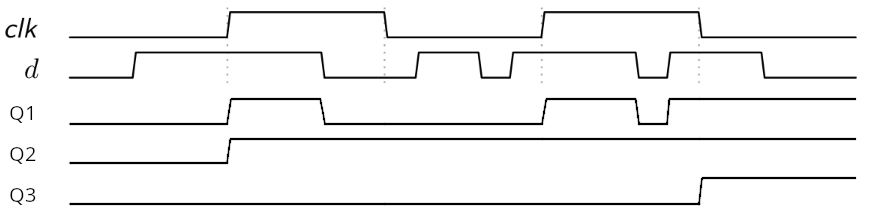
\includegraphics[scale=0.3]{./L06Z01.png}
\end{center}
\section{Narysuj asynchroniczny przerzutnik RS w wersji dualnej do przedstawionej na wykładzie (tzn. z bramkami NAND zamiast NOR). Narysuj jego tabelę charakterystyczną oraz przykładowe przebiegi sygnałów.}
\textbf{asynchroniczny przerzutnik RS}. Słowo asynchroniczny precyzuje nam że przerzutnik jest bez zegara, zależny bezpośrednio od wejścia.
\begin{center}
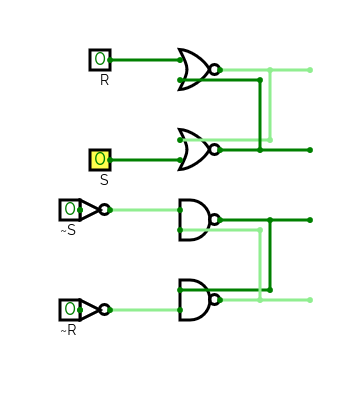
\includegraphics[scale=0.3]{./L06Z02.png}
\end{center}
\section{Zaprojektuj obwód wykorzystujący przerzutniki typu D, który dla sygnału wejściowego będącego falą prostokątną o częstotliwości f, wygeneruje falę prostokątną o częstotliwości f/4}
\begin{center}
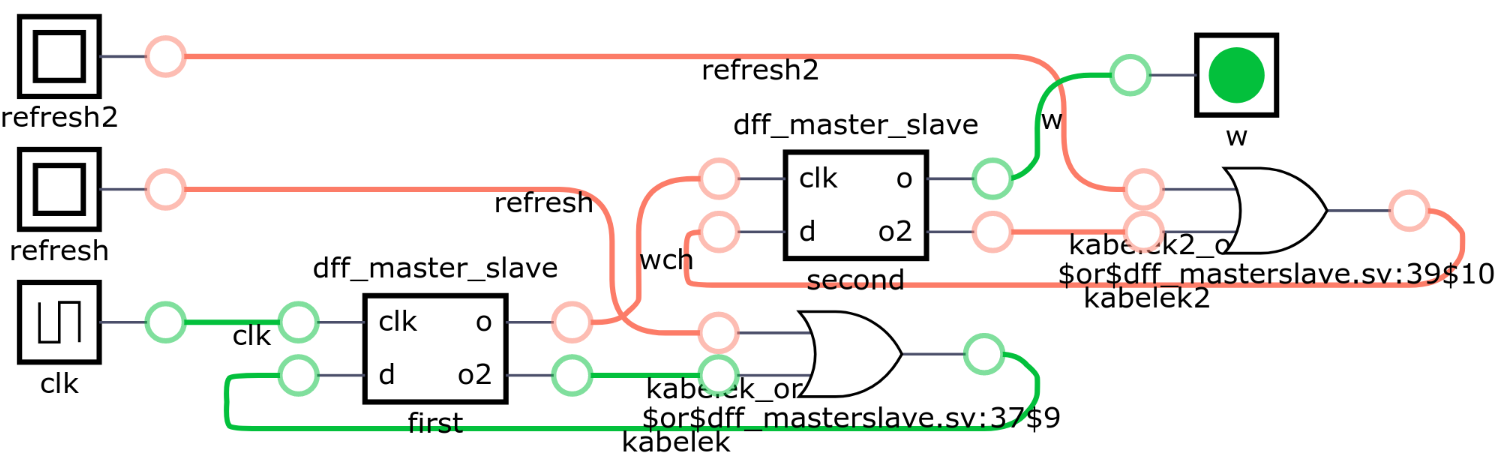
\includegraphics[scale=0.3]{./L06Z03.png}
\end{center}
\section{Przerzutnik synchroniczny typu RS zachowuje się w nieprzewidywalny sposób, gdy zarówno wejście s oraz r są w stanie wysokim w momencie zmiany stanu wejścia en z wysokiego na niski. Jedną z metod poradzenia sobie z tym jest zmodyfikowanie przerzutnika tak, aby w takiej sytuacji zachowywał się tak samo, jak gdyby wyłacznie wejście s było w stanie wysokim. Narysuj taki przerzutnik. Jaka sytuacja może wprowadzić w stan metastabilny zmodyfikowany przerzutnik?}
\begin{center}
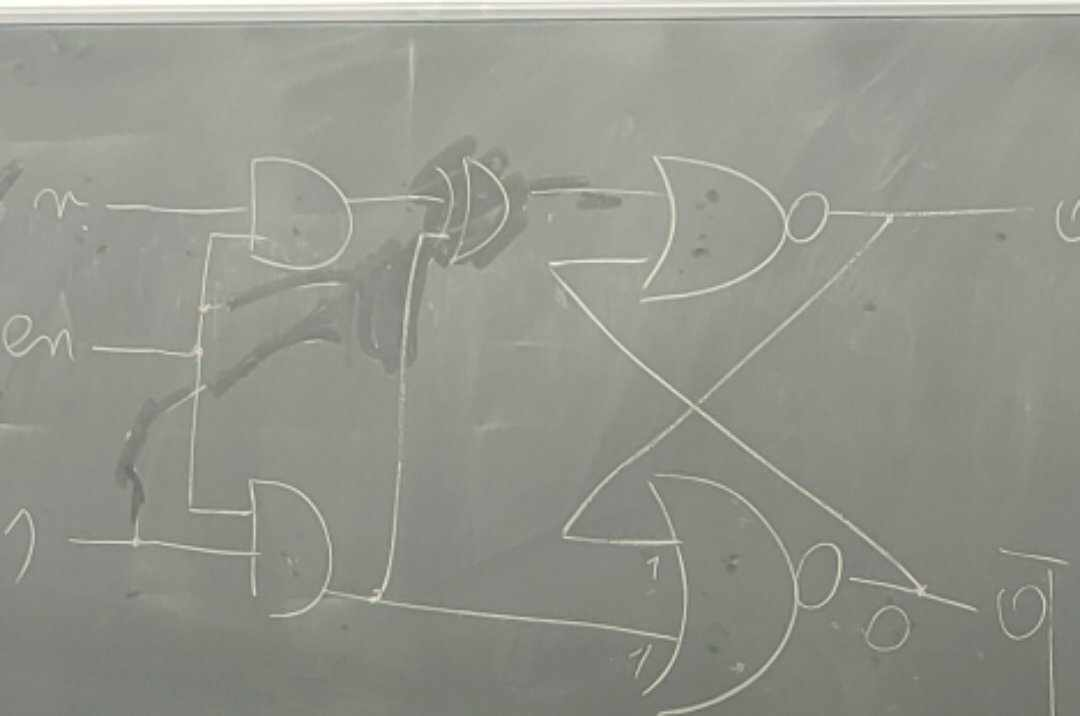
\includegraphics[scale=0.3]{./L06Z04.jpg}
\end{center}

\section{Pokaż, jak skonstruować przerzutnik typu JK używając przerzutnika typu T i dodatkowych bramek.}
\textbf{Przerzutnik typu T} to taki przerzutnik, który dla zapalonego t dokonuje negacji co każde wzrastające zbocze.\\
\textbf{JK} natomiast jeszcze daje możliwość ustawienia wartości w przypadku kiedy dwa wejściowe bity są przeciwne.
\begin{center}
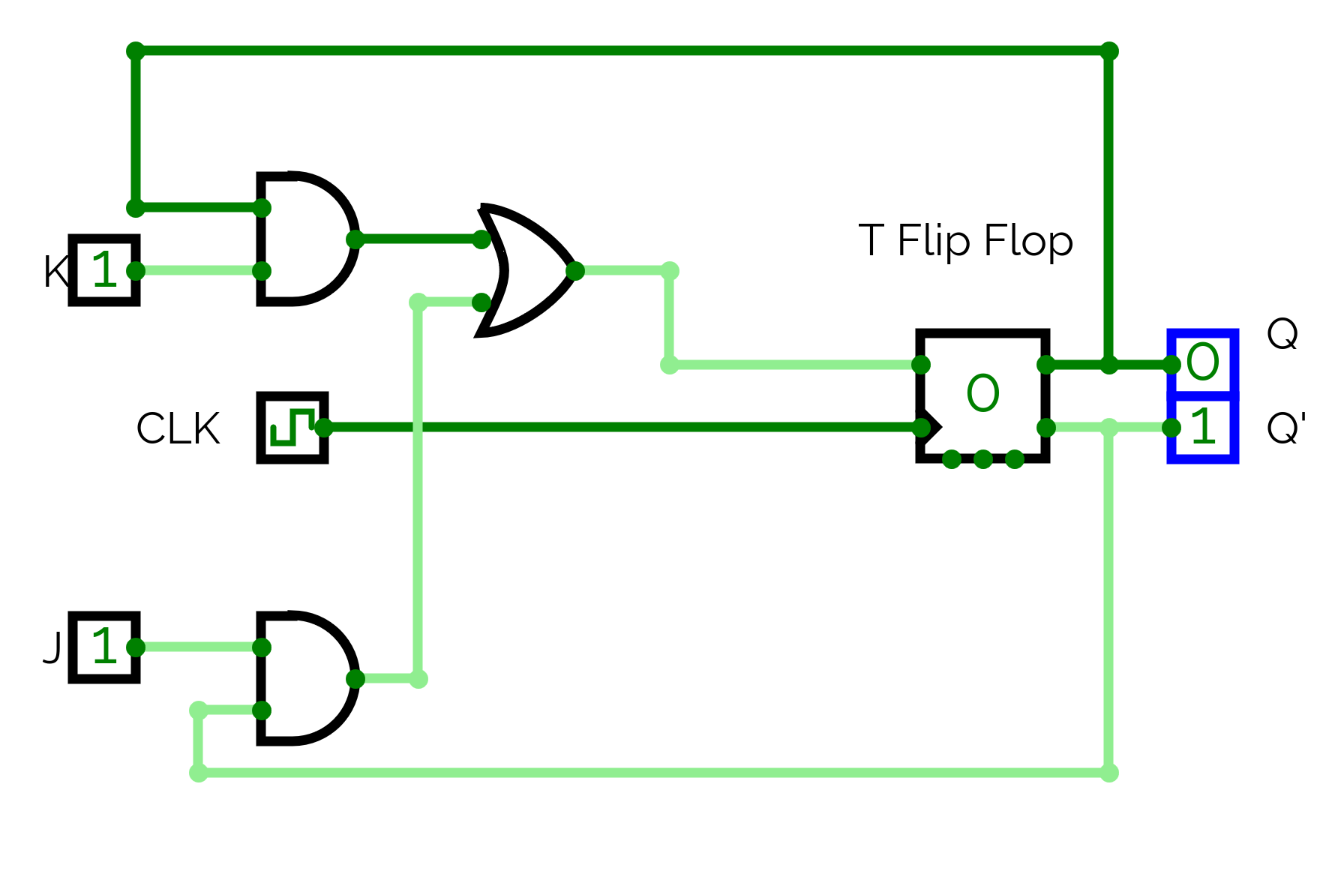
\includegraphics[scale=0.3]{./L06Z05.png}
\end{center}
\section{Uniwersalny rejestr przesuwny może ładować bity zarówno od lewej, jak i od prawej strony, może też ładować je równolegle. Zaprojektuj 4-bitowy rejestr tego typu.}
TODO
\section{Zaprojektuj 4-bitowy rejestr, który posiada następujące funkcje, wykonywane na zboczu narastającym zegara, wybierane za pomocą bitów sterujących $s_0$ i $s_1$}
\begin{center}
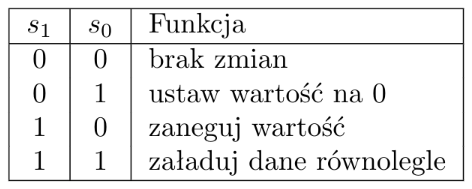
\includegraphics[scale=0.3]{./L06Z07.png}
\end{center}
\end{document}